\documentclass[10pt]{beamer}
\usetheme{Madrid}
\usecolortheme{default}

\usepackage[utf8]{inputenc}
\usepackage{amsmath,amssymb}
\usepackage{algorithm,algorithmicx,algpseudocode}
\usepackage{booktabs}
\usepackage{tikz}
\usepackage{colortbl}

\title[DP-GCD]{High-Dimensional Private Empirical Risk Minimization\\\\by Greedy Coordinate Descent}
\author{Pierre Cornilleau and Mohamed Amine Belkasmi}
\institute{Université Paris-Dauphine}
\date{}

\begin{document}

\frame{\titlepage}

\begin{frame}{Outline}
\tableofcontents
\end{frame}

\section{Motivation}

\begin{frame}{The Privacy–Utility Trade-off}
\begin{columns}[T]
\column{0.5\textwidth}
\textbf{Why privacy is crucial}
\begin{itemize}
\item Medical records
\item Financial data
\item Personal information
\item Legal requirements
\end{itemize}

\vspace{1em}
\textbf{The Problem}
\begin{itemize}
\item Leakage of training data
\item Membership inference attacks
\item Model inversion attacks
\end{itemize}

\column{0.5\textwidth}
\begin{center}
% Make sure you have the image privacy_tradeoff.png in your folder
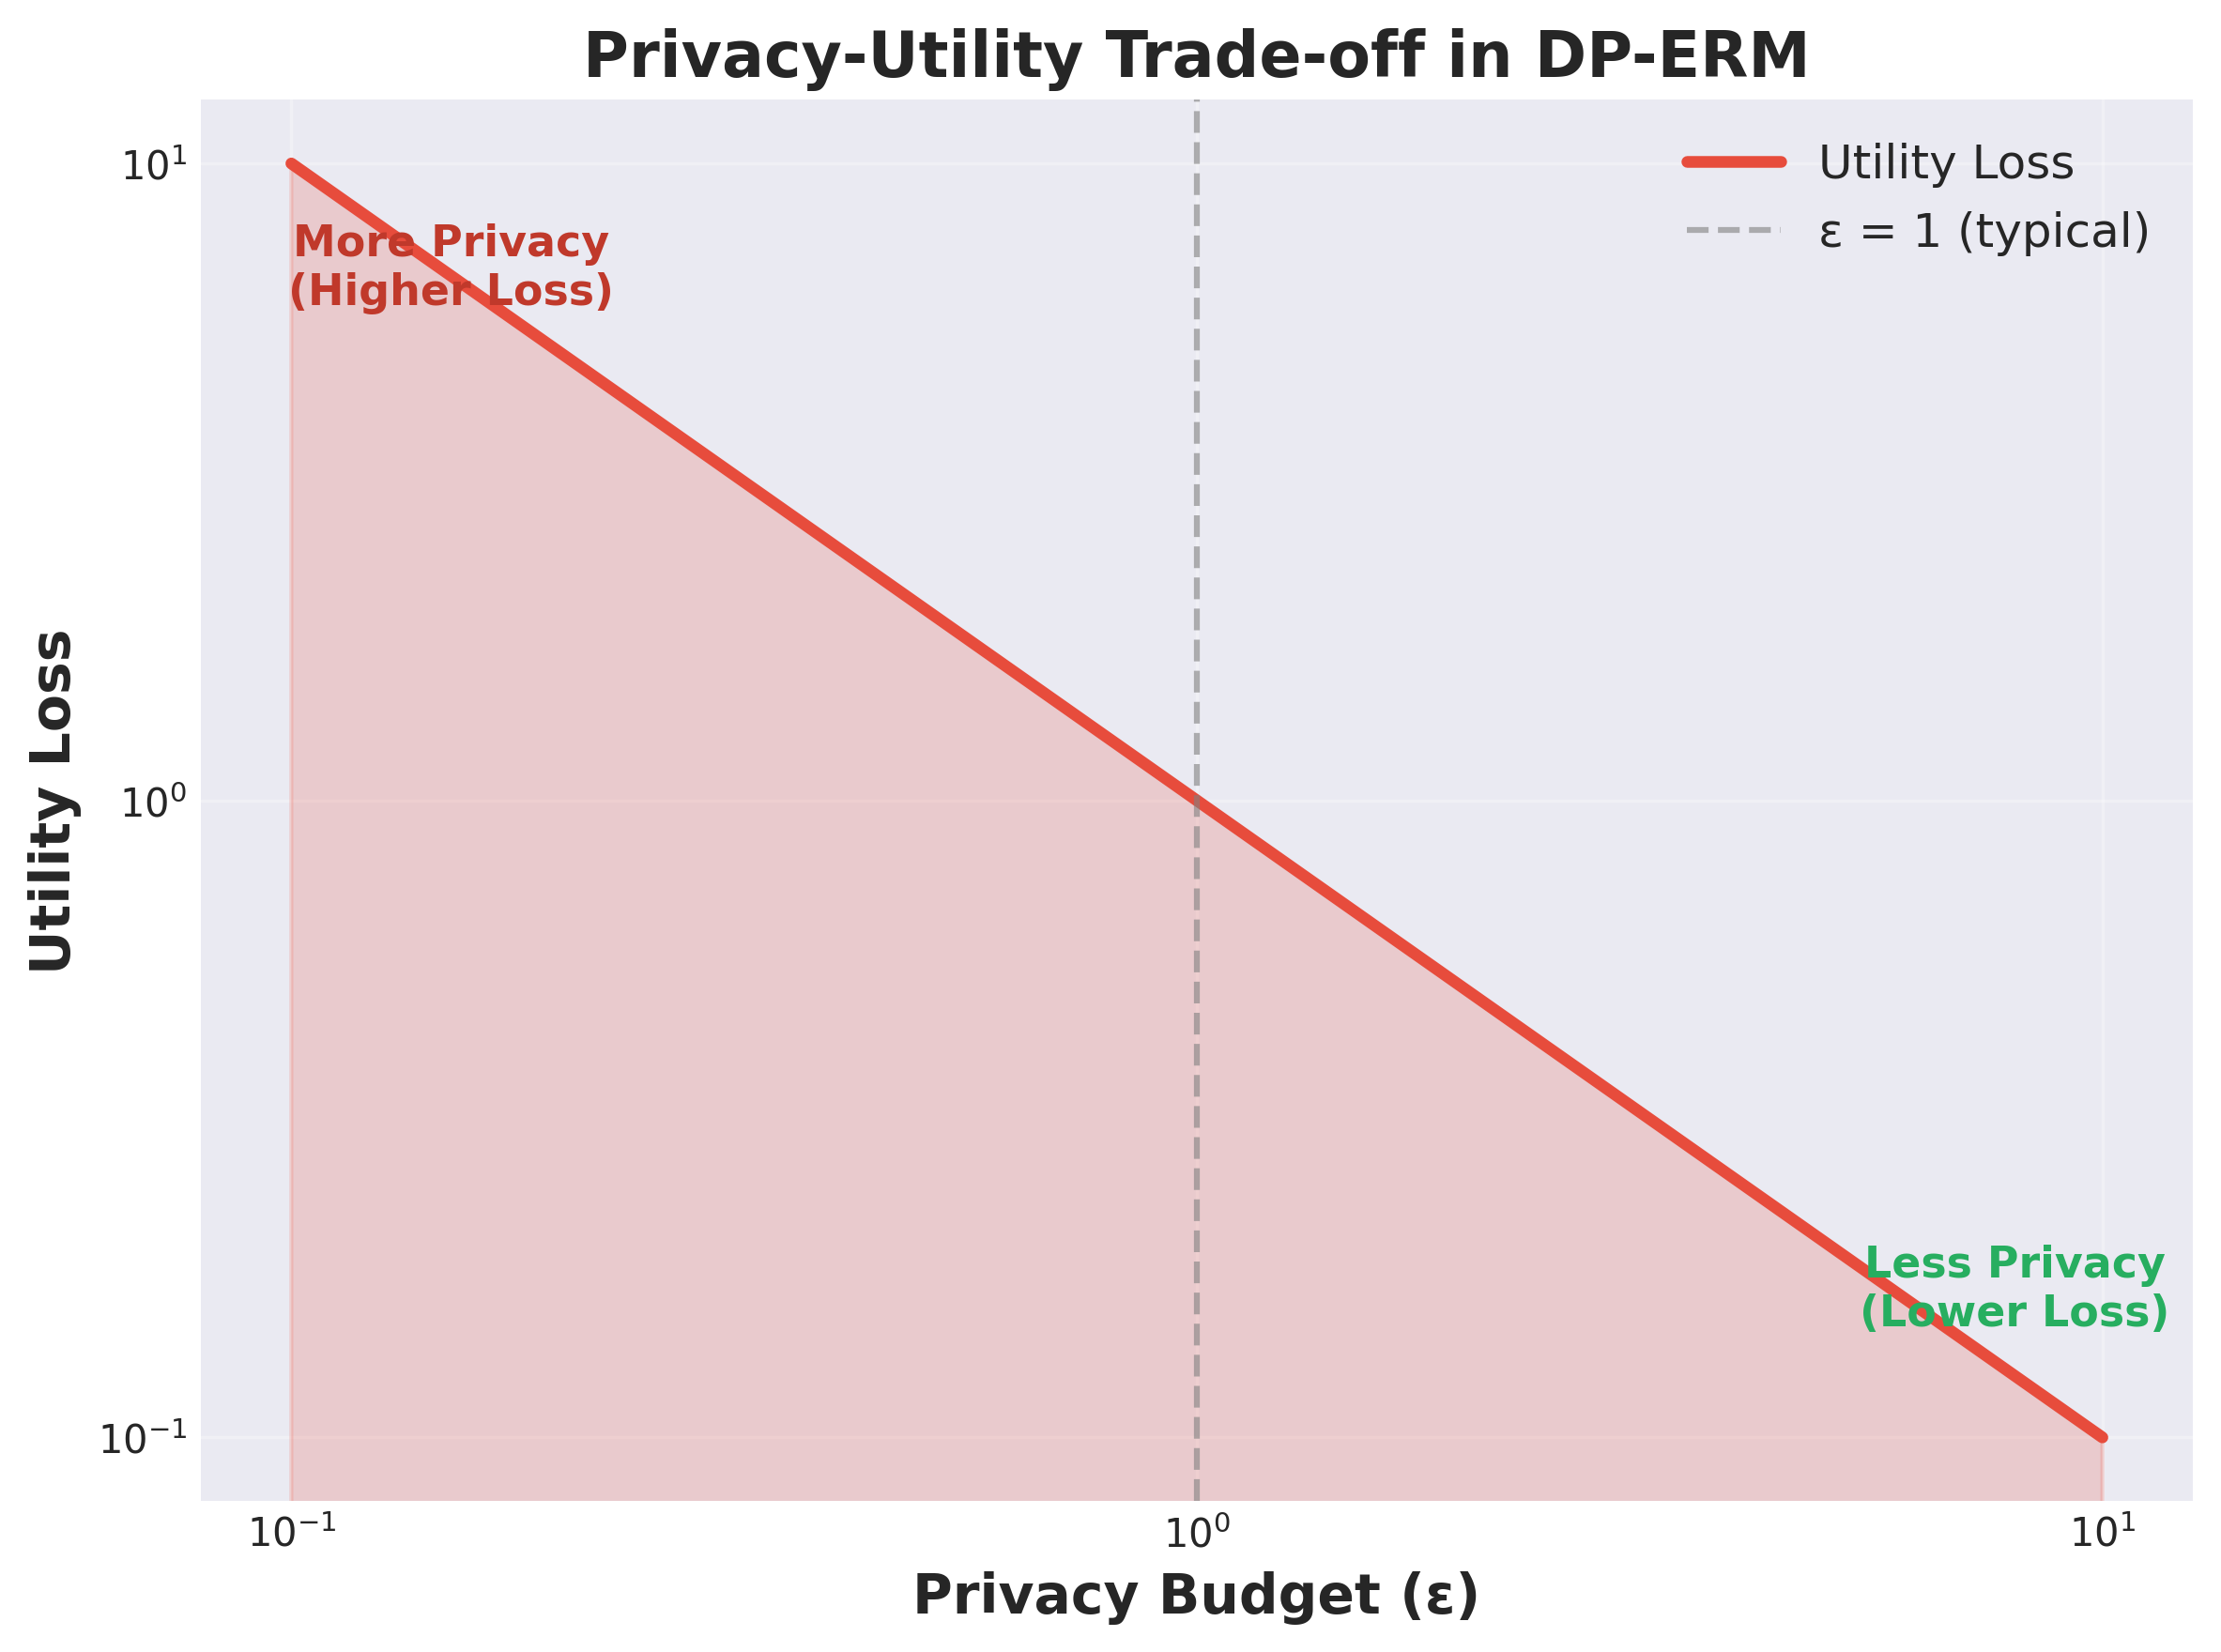
\includegraphics[width=0.9\textwidth]{privacy_tradeoff.png} 
\end{center}
\vspace{0.5em}
\textbf{Differential Privacy (DP)} provides rigorous guarantees but at a certain cost...
\end{columns}
\end{frame}

\begin{frame}{The Curse of Dimensionality in DP-ERM}
\textbf{Standard Problem:}
\[
w^\star \in \arg\min_{w \in \mathbb{R}^p} \underbrace{\frac{1}{n} \sum_{i=1}^n \ell(w; d_i)}_{f(w)}
\]

\vspace{1em}
\textbf{Known Results:}
\begin{itemize}
\item Bassily et al. (2014): The utility of DP-ERM degrades \alert{polynomially} with the dimension $p$.
\item For high-dimensional problems ($p \gg n$): \textbf{catastrophic loss of utility}.
\end{itemize}

\vspace{1em}
\begin{block}{The Challenge}
Can we obtain a \alert{logarithmic} dependence on $p$ instead of a polynomial one?
\end{block}
\end{frame}

\begin{frame}{Previous Approaches and Limitations}
\begin{table}
\footnotesize
\begin{tabular}{@{}lll@{}}
\toprule
\textbf{Approach} & \textbf{Dependence on Dimension} & \textbf{Limitation} \\
\midrule
DP-SGD & $\tilde{O}(p / n^{2/3}\varepsilon^{2/3})$ & Polynomial in $p$ \\
DP-Frank-Wolfe & $\tilde{O}(\log p / n^{2/3}\varepsilon^{2/3})$ & Requires an $\ell_1$ constraint \\
Sparse regression & $\tilde{O}(\log p)$ & Sparsity assumed known \\
Public data & $\tilde{O}(\log p)$ & Requires public data \\
\bottomrule
\end{tabular}
\end{table}

\vspace{1em}
\begin{alertblock}{The Gap}
No algorithm achieves a $\log p$ dependence for \emph{unconstrained} problems without prior knowledge of structure.
\end{alertblock}
\end{frame}

\section{Background}

\begin{frame}{Reminder: Differential Privacy}
\begin{definition}[($\varepsilon, \delta$)-DP]
An algorithm $\mathcal{A}$ is $(\varepsilon, \delta)$-DP if for all neighboring datasets $D, D'$ (differing in one record):
\[
\Pr[\mathcal{A}(D) \in S] \leq e^\varepsilon \Pr[\mathcal{A}(D') \in S] + \delta
\]
\end{definition}

\vspace{1em}
\textbf{Key Mechanisms Used:}
\begin{itemize}
\item \textbf{Laplace:} Add noise $\sim \text{Lap}(\Delta_1 / \varepsilon)$ to a query with $\ell_1$-sensitivity $\Delta_1$.
\item \textbf{Report-Noisy-Max:} Perturbs each entry and returns the index of the maximum.
\begin{itemize}
\item Reveals only \alert{one single number} (the index) instead of $p$ values.
\item Exponential savings in the privacy budget!
\end{itemize}
\end{itemize}
\end{frame}

\begin{frame}{Basics of Coordinate Descent (CD)}
\textbf{Standard Gradient Descent:}
\[
w^{t+1} = w^t - \gamma \nabla f(w^t) \quad \text{(updates all $p$ coordinates)}
\]

\vspace{1em}
\textbf{Coordinate Descent:}
\[
w^{t+1} = w^t - \gamma_j [\nabla f(w^t)]_j \cdot e_j \quad \text{(updates only coordinate $j$)}
\]

\vspace{1em}
\begin{columns}[T]
\column{0.5\textwidth}
\textbf{Random Selection}
\begin{itemize}
\item Choose $j$ uniformly at random
\item Simple, unbiased
\item May waste updates
\end{itemize}

\column{0.5\textwidth}
\textbf{Greedy Selection}
\begin{itemize}
\item Choose $j$ maximizing $|\nabla_j f|$
\item Faster convergence
\item Exploits the structure of the problem
\end{itemize}
\end{columns}
\end{frame}

\section{The DP-GCD Algorithm}

\begin{frame}{Algorithm Overview}
\begin{algorithm}[H]
\caption{DP-GCD (Simplified)}
\footnotesize
\begin{algorithmic}[1]
\State \textbf{Input:} $w^0 \in \mathbb{R}^p$, iterations $T$, noise scales $\{\lambda_j, \lambda_j'\}$
\For{$t = 0$ to $T-1$}
    \State \alert{Greedy selection (private via Report-Noisy-Max):}
    \[j_t \leftarrow \arg\max_{j' \in [p]} \left\{ \frac{|\nabla_{j'} f(w^t) + \chi_{j'}^t|}{\sqrt{M_{j'}}} \right\} \quad \text{with } \chi_{j'}^t \sim \text{Lap}(\lambda_{j'}')\]
    \State \alert{Single-coordinate update:} 
    \[w^{t+1} \leftarrow w^t - \gamma_{j_t} (\nabla_{j_t} f(w^t) + \eta_{j_t}^t) e_{j_t} \quad \text{with } \eta_{j_t}^t \sim \text{Lap}(\lambda_{j_t})\]
\EndFor
\State \textbf{Return} $w^T$
\end{algorithmic}
\end{algorithm}

\vspace{0.5em}
\textbf{Key idea:} Concentrate the privacy budget on the \emph{most informative} coordinates.
\end{frame}

\begin{frame}{Why Greedy Selection Helps Privacy}

\textbf{Dependence on dimension in private optimization}

\begin{itemize}

\item \textbf{DP-SGD:} Privatizes the full gradient $\Rightarrow$ noise $ \propto \sqrt{p}$ or $p$.

\item \textbf{DP-GCD:}
\begin{itemize}
    \item Report-Noisy-Max selects the coordinate.
    \item Privatizes \alert{only one coordinate per step}.
\end{itemize}

\item \textbf{Result:} The dependence on dimension goes from $\sqrt{p}, p \rightarrow \alert{\log p}$.

\end{itemize}

\vspace{1em}
\begin{block}{Intuition}
For sparse or quasi-sparse problems, only $s \ll p$ coordinates matter.\\\\
DP-GCD finds and updates them automatically.
\end{block}

\end{frame}

\begin{frame}{Privacy Guarantees}
\begin{theorem}[Privacy (Theorem 4.2)]
With noise scales:
\[
\lambda_j = \lambda_j' = \frac{8L_j}{n\varepsilon} \sqrt{T \log(1/\delta)}
\]
DP-GCD satisfies $(\varepsilon, \delta)$-differential privacy.
\end{theorem}

\vspace{1em}
\textbf{Proof sketch:}
\begin{itemize}
\item Each iteration accesses the data twice: (1) coordinate selection, (2) computation of the gradient entry.
\item Each access is $\varepsilon/(16\sqrt{2T\log(1/\delta)})$-DP via the Laplace mechanism.
\item The advanced composition theorem over $2T$ mechanisms ensures an overall $(\varepsilon, \delta)$-DP level.
\end{itemize}

\end{frame}

\section{Theoretical Results}

\begin{frame}{Main Utility Results}
\begin{theorem}[Utility (Theorem 4.4, Simplified)]
Let
$R_{M,1} = \max_{w \in \mathbb{R}^p} \; \max_{w^* \in W^*} \left\{ \|w - w^*\|_{M,1} \;\middle|\; f(w) \le f(w_0) \right\}$
. With probability at least $1 - \zeta$:

\vspace{0.5em}
\textbf{Convex case:}
\[
f(w_{\text{priv}}) - f^\star =
\tilde{O}\!\left(
\frac{R_{M,1}^{4/3} L_{\max}^{2/3} \log(1/\delta)\,\log(p/\zeta)}
{n^{2/3} \varepsilon^{2/3} M_{\min}^{1/3}}
\right)
\]

\textbf{Strongly convex case:}
\[
f(w_{\text{priv}}) - f^\star =
\tilde{O}\!\left(
\frac{L_{\max}^{2}\,\log(1/\delta)\,\log\!\left(\frac{2p}{\mu_M \zeta}\right)}
{M_{\min}\,\mu_{M,1}^{2}\,n^{2} \varepsilon^{2}}
\right)
\]
\end{theorem}

\vspace{1em}
\begin{alertblock}{Major Achievement}
\alert{Logarithmic} dependence on $p$ (and not polynomial).
\end{alertblock}
\end{frame}

\begin{frame}{Comparison with Previous Work}
\begin{table}
\footnotesize
\begin{tabular}{@{}lccc@{}}
\toprule
\textbf{Algorithm} & \textbf{Convex} & \textbf{Strongly Convex} & \textbf{Constraint} \\
\midrule
DP-SGD & $\tilde{O}(p/n^{2/3}\varepsilon^{2/3})$ & $\tilde{O}(p/n^2\varepsilon^2)$ & None \\
DP-FW & $\tilde{O}(\log p/n^{2/3}\varepsilon^{2/3})$ & $\tilde{O}(\log p^{4/3}/n^{4/3}\varepsilon^{4/3})$ & $\ell_1$ ball \\
\rowcolor{yellow!30}
DP-GCD & $\tilde{O}(\log p/n^{2/3}\varepsilon^{2/3})$ & $\alert{\tilde{O}(\log p/n^2\varepsilon^2)}$ & \textbf{None} \\
\bottomrule
\end{tabular}
\end{table}

\vspace{1em}
\textbf{DP-GCD advances:}
\begin{itemize}
\item Matches DP-FW without needing to constrain the space via $\ell_1$.
\item \alert{First} algorithm to achieve $\tilde{O}(\log p / n^2\varepsilon^2)$ in the strongly convex case.
\item Applicable to general unconstrained problems.
\end{itemize}
\end{frame}

\begin{frame}{Adaptation to Quasi-Sparsity}

\begin{definition}[($\alpha,\tau$)-Quasi-Sparsity]
A vector $w \in \mathbb{R}^p$ is $(\alpha,\tau)$-quasi-sparse if at most $\tau$ coordinates satisfy
\[
|w_j| > \alpha .
\]
When $\alpha = 0$, the vector is strictly $\tau$-sparse.
\end{definition}

\vspace{1em}

\begin{theorem}[Theorem 4.7, Simplified]
Assume $f$ is strongly convex ($\mu_{M,2}$) and the optimal solution is $(\alpha,\tau)$-quasi-sparse.
If DP-GCD is initialized at $w^0=0$ and the iterates remain $s$-sparse, then with high probability; \text{(simplified bound under additional assumptions)}
\[
f(w^T) - f^\star
=
\tilde{O}\!\left(
\frac{L_{\max}^2}{M_{\min}}
\frac{(s+\tau)^2 \log(2p/\zeta)}{\mu_{M,2} n^2 \varepsilon^2}
\right).
\]
\end{theorem}

\end{frame}

\begin{frame}{Follow-up}

\vspace{1em}

\begin{alertblock}{Main Idea}
When the solution is dominated by a few coordinates, the effective dimension becomes
\[
p \;\rightarrow\; (s+\tau),
\]
so DP-GCD automatically adapts to quasi-sparsity.
\end{alertblock}

\vspace{1em}
\textbf{Impact:} The dependence shifts from ambient $p$ to an effective ratio of \alert{$(s+\tau)^2$}.

\vspace{0.5em}
\textbf{Crucial:} DP-GCD \emph{automatically} adapts without knowing $s$ beforehand!
\end{frame}

\begin{frame}{How DP-GCD Exploits Structure}
\begin{center}
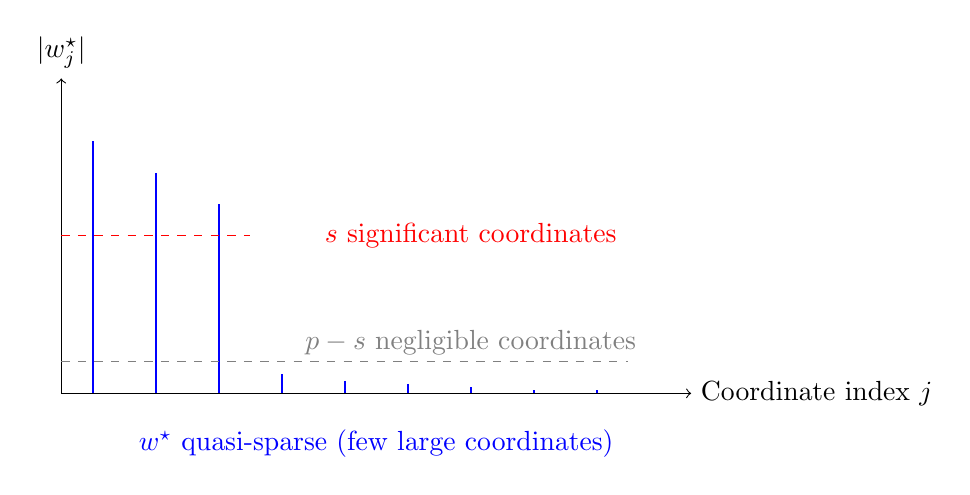
\begin{tikzpicture}[scale=0.8]
% Coordinate axis
\draw[->] (0,0) -- (10,0) node[right] {Coordinate index $j$};
\draw[->] (0,0) -- (0,5) node[above] {$|w_j^\star|$};

% Quasi-sparse solution
\draw[thick, blue] (0.5,4) -- (0.5,0);
\draw[thick, blue] (1.5,3.5) -- (1.5,0);
\draw[thick, blue] (2.5,3) -- (2.5,0);
\draw[thick, blue] (3.5,0.3) -- (3.5,0);
\draw[thick, blue] (4.5,0.2) -- (4.5,0);
\draw[thick, blue] (5.5,0.15) -- (5.5,0);
\draw[thick, blue] (6.5,0.1) -- (6.5,0);
\draw[thick, blue] (7.5,0.05) -- (7.5,0);
\draw[thick, blue] (8.5,0.05) -- (8.5,0);

\node[blue] at (5, -0.8) {$w^\star$ quasi-sparse (few large coordinates)};

% Annotations
\draw[dashed, red] (0,2.5) -- (3,2.5);
\node[red] at (6.5, 2.5) {$s$ significant coordinates};
\draw[dashed, gray] (0,0.5) -- (9,0.5);
\node[gray] at (6.5, 0.8) {$p - s$ negligible coordinates};

\end{tikzpicture}
\end{center}

\textbf{DP-GCD behavior:}
\begin{itemize}
\item Greedy selection first targets the large coordinates.
\item Iterates remain sparse if $w^0 = 0$.
\item Converges in fewer iterations.
\end{itemize}
\end{frame}

\section{Experiments}

\begin{frame}{Experimental Setup}
\begin{table}
\scriptsize
\begin{tabular}{@{}lccl@{}}
\toprule
\textbf{Dataset} & $n$ & $p$ & \textbf{Notes} \\
\midrule
log1, log2 & 1 000 & 100 & Synthetic, quasi-sparse \\
square & 1 000 & 1 000 & Synthetic, 10 non-zeros \\
california & 20 640 & 8 & Real, low dimension \\
madelon & 2 600 & 501 & Real \\
dorothea & 800 & \alert{88 119} & Real, very high dimension \\
\bottomrule
\end{tabular}
\end{table}

\vspace{1em}
\textbf{Algorithms compared:}
\begin{itemize}
\item \textbf{DP-SGD:} Batch size 1, Gaussian mechanism.
\item \textbf{DP-CD:} Random selection of coordinates.
\item \textbf{DP-GCD:} Greedy selection of coordinates (our approach).
\end{itemize}

\vspace{0.5em}
\textbf{Privacy budget:} $\varepsilon = 1$, $\delta = 1/n^2$.

\vspace{0.5em}
\textbf{Metric:} Relative error $(f(w^t) - f^\star) / f^\star$ versus passes over the data.
\end{frame}

\begin{frame}{Key Experimental Results}
\begin{columns}[T]
\column{0.5\textwidth}
\textbf{High-dimensional sparse (dorothea)}
\begin{itemize}
\item DP-GCD: Only algorithm that \alert{converges}.
\item DP-SGD/DP-CD: Fail to decrease the objective.
\item $p = 88k$: Dramatic advantage.
\end{itemize}

\vspace{1em}
\textbf{Quasi-sparse (log2, madelon)}
\begin{itemize}
\item DP-GCD: Convergence about $2$ to $3\times$ faster.
\item Reaches error $10^{-7}$ versus $10^{-5}$ for others.
\end{itemize}

\column{0.5\textwidth}
\textbf{Low dimension (california)}
\begin{itemize}
\item DP-GCD: Comparable to DP-SGD.
\item Greedy selection overhead not justified here.
\item $p = 8$: No sparsity to exploit.
\end{itemize}

\vspace{1em}
\textbf{Computational cost}
\begin{itemize}
\item 1 DP-GCD iteration = one full gradient.
\item Equivalent to $p$ iterations of DP-CD.
\item Largely justified by the utility gain per pass.
\end{itemize}
\end{columns}

\vspace{1em}
\begin{alertblock}{Takeaway}
DP-GCD excels on high-dimensional problems with (quasi-)sparse structure.
\end{alertblock}
\end{frame}

\begin{frame}{Visualization: log2 Results}
\begin{center}
% Make sure you have the image log2_results.png in your folder

\includegraphics[width=0.85\textwidth]{log2_results.png}
\end{center}

\vspace{-0.5em}
\scriptsize
\textbf{Observation:} DP-GCD (blue) converges much faster than DP-CD (red) and DP-SGD (green) on a quasi-sparse logistic regression problem.
\end{frame}

\section{Critical Analysis}

\begin{frame}{Strengths}
\begin{enumerate}
\item \textbf{No domain constraint}
\begin{itemize}
\item Works on unconstrained problems.
\end{itemize}

\item \textbf{Automatic adaptation}
\begin{itemize}
\item Exploits quasi-sparsity without prior knowledge of $s$.
\end{itemize}

\item \textbf{Logarithmic dependence}
\begin{itemize}
\item Achieves $\tilde{O}(\log p)$ in favorable settings.
\end{itemize}

\item \textbf{Per-coordinate adaptivity}
\begin{itemize}
\item Uses coordinate-specific Lipschitz constants $L_j$ to calibrate noise.
\end{itemize}

\item \textbf{Optimal rates for strongly convex problems}
\begin{itemize}
\item $\tilde{O}(\log p / n^2\varepsilon^2)$ achieved without complex heuristics.
\end{itemize}

\item \textbf{Strong empirical validation}
\begin{itemize}
\item Spectacular improvements on dorothea ($p = 88k$).
\end{itemize}
\end{enumerate}
\end{frame}

\begin{frame}{Limitations}
\begin{enumerate}
\item \textbf{Computational cost}
\begin{itemize}
\item 1 DP-GCD iteration = 1 full pass over the data.
\item Equivalent to $p$ iterations of DP-CD or $n$ iterations of DP-SGD.
\item Higher per-iteration cost, but often fewer iterations needed.
\end{itemize}

\item \textbf{Proximal extension without proven theory}
\begin{itemize}
\item Authors propose a proximal variant for $\ell_1$ regularization.
\item \alert{No utility analysis is provided for this variant} in the paper.
\item Proximal greedy CD is already complex without privacy constraints.
\end{itemize}

\item \textbf{Required assumptions}
\begin{itemize}
\item Requires bounds on coordinate-wise Lipschitz/smoothness constants.
\item Lower bound on the initial gap required: $f(w^0) - f^\star \geq \Omega(\dots)$.
\end{itemize}

\end{enumerate}
\end{frame}

\begin{frame}{Limitations (cont.)}
\begin{enumerate}
\setcounter{enumi}{3}

\item \textbf{Not optimal in all regimes}
\begin{itemize}
\item When $\ell_2$-norm quantities are bounded, the algorithm does not always perfectly match DP-SGD in the worst case.
\end{itemize}

\item \textbf{Privacy budget overhead}
\begin{itemize}
\item Report-Noisy-Max consumes budget to select the coordinate.
\item In low dimension, this cost outweighs the benefits.
\end{itemize}

\item \textbf{Limited to smooth objectives}
\begin{itemize}
\item Main theory relies on smooth loss functions.
\item Extensions to non-smooth parameters remain open directions.
\end{itemize}
\end{enumerate}

\vspace{1em}
\begin{block}{When to use DP-GCD?}
For high-dimensional problems suspected to be quasi-sparse, where final model accuracy prevails over raw computation time.
\end{block}
\end{frame}

\section{Conclusion}

\begin{frame}{Summary}
\textbf{Main Contributions:}
\begin{enumerate}
\item \textbf{DP-GCD algorithm:} Greedy coordinate descent with Report-Noisy-Max.
\item \textbf{Theoretical guarantees:} $\tilde{O}(\log p)$ utility for unconstrained problems.
\item \textbf{Automatic adaptation:} Exploits quasi-sparsity without manual prior tuning.
\item \textbf{Empirical validation:} Clear advantages on high-dimensional datasets.
\end{enumerate}

\vspace{1em}
\textbf{Key Idea:}
\begin{block}{}
By focusing the privacy budget on the \alert{most informative} coordinates, DP-GCD drastically mitigates the effect of high dimension.
\end{block}

\vspace{1em}
\textbf{Potential impact:} Paves the way for private and efficient learning in genomics, NLP, or finance (e.g., trading floor models).
\end{frame}

\begin{frame}{Open Questions}
\begin{enumerate}
\item \textbf{Proximal analysis:} Can we formally prove the utility of the proximal variant for non-smooth regularizers?

\item \textbf{Universal algorithm:} Is there an algorithm offering optimal utility for \emph{all} norm regimes ($\ell_1$ and $\ell_2$)?

\item \textbf{Computational efficiency:} How can we reduce the $O(np)$ per-iteration cost while preserving privacy guarantees?

\item \textbf{Deep learning extensions:} How does DP-GCD behave on non-convex problems (e.g., neural networks)?
\end{enumerate}

\vspace{1em}
\begin{alertblock}{Research Direction}
Develop adaptive algorithms combining the advantage of DP-GCD with the stochastic speed of DP-SGD.
\end{alertblock}
\end{frame}

\begin{frame}[standout]
\Huge Thank you!
\vspace{2em}

\normalsize
Any questions?

\vspace{2em}
\footnotesize
\textit{Mangold, P., Bellet, A., Salmon, J., and Tommasi, M.\\\\
High-Dimensional Private Empirical Risk Minimization\\\\
by Greedy Coordinate Descent. AISTATS 2023.}
\end{frame}

\appendix

\begin{frame}[allowframebreaks]{Appendix: Technical Details}
\textbf{Coordinate-Wise Regularity Assumptions}

\vspace{0.5em}
\textbf{Component-wise smoothness:}
\[
f(w) \leq f(v) + \langle \nabla f(v), w - v \rangle + \frac{1}{2} \|w - v\|_{M,2}^2
\]
where $\|w\|_{M,2}^2 = \sum_{j=1}^p M_j w_j^2$.

\vspace{0.5em}
\textbf{Lipschitz constants:} For each $j$,
\[
|f(w + t e_j) - f(w)| \leq L_j |t|
\]

\vspace{0.5em}
\textbf{Strong convexity with respect to the $\ell_1$ norm:}
\[
f(w) \geq f(v) + \langle \nabla f(v), w - v \rangle + \frac{\mu_{M,1}}{2} \|w - v\|_{M,1}^2
\]

\framebreak

\textbf{Report-Noisy-Max Mechanism}

\vspace{0.5em}
Given scores $\{q_1, \ldots, q_p\}$ with respective $\ell_1$-sensitivities $\{\Delta_1, \ldots, \Delta_p\}$:
\[
j^\star = \arg\max_{j \in [p]} \{q_j + \text{Lap}(\Delta_j / \varepsilon)\}
\]

\textbf{Privacy guarantee:} $\varepsilon$-DP (pure).

\textbf{Why it is powerful:} This mechanism reveals only the index (one number), hiding the associated $p$ values.

\framebreak

\textbf{Proof Sketch: Utility (Convex Case)}

\vspace{0.5em}
\textbf{Noisy descent lemma:}
\[
f(w^{t+1}) - f(w^t) \leq -\frac{1}{2M_j} |\nabla_j f(w^t)|^2 + \text{noise terms}
\]

\vspace{0.5em}
\textbf{Key property:} Greedy selection ensures that
\[
\frac{1}{M_j} |\nabla_j f(w^t)|^2 \geq \frac{\|\nabla f(w^t)\|^2}{2 \sum_{j'} M_{j'}}
\]

\vspace{0.5em}
Thus, either:
\begin{itemize}
\item $w^t$ is far from optimum $\Rightarrow$ guaranteed progress despite noise.
\item $w^t$ is close to optimum $\Rightarrow$ the algorithm stagnates in a small controlled region.
\end{itemize}

Balancing these two regimes together with Chernoff bounds yields the result.
\end{frame}

\begin{frame}{Appendix: Synthetic Data Generation}
\textbf{log1 / log2:}
\begin{itemize}
\item $X \in \mathbb{R}^{1000 \times 100}$, columns $\sim \mathcal{N}(0, 1)$.
\item $w_{\text{true}} \sim \text{LogNormal}(0, \sigma)$ with $\sigma \in \{1, 2\}$.
\item Logistic: $y_i \sim \text{Bernoulli}(\sigma(x_i^\top w_{\text{true}} + \xi_i))$.
\item The LogNormal law enforces quasi-sparsity (few large values, many small ones).
\end{itemize}

\vspace{1em}
\textbf{square:}
\begin{itemize}
\item $X \in \mathbb{R}^{1000 \times 1000}$, columns $\sim \mathcal{N}(0, 1)$.
\item $w_{\text{true}}$ has exactly 10 non-zero entries (at random).
\item $y = X w_{\text{true}} + \xi$ with $\xi \sim \mathcal{N}(0, \sigma^2)$.
\item LASSO regression (least squares + $\ell_1$ penalty).
\end{itemize}
\end{frame}

\end{document}
